\documentclass{exam}
\usepackage{xcolor, minted, graphicx, fontspec}
\setmainfont{Open Sans}
\graphicspath{ {./images} }

\author{Jordy Alkema}
\title {Homework Week 3}

\begin{document}
\maketitle

\section{Questions}
\begin{questions}
	\question
	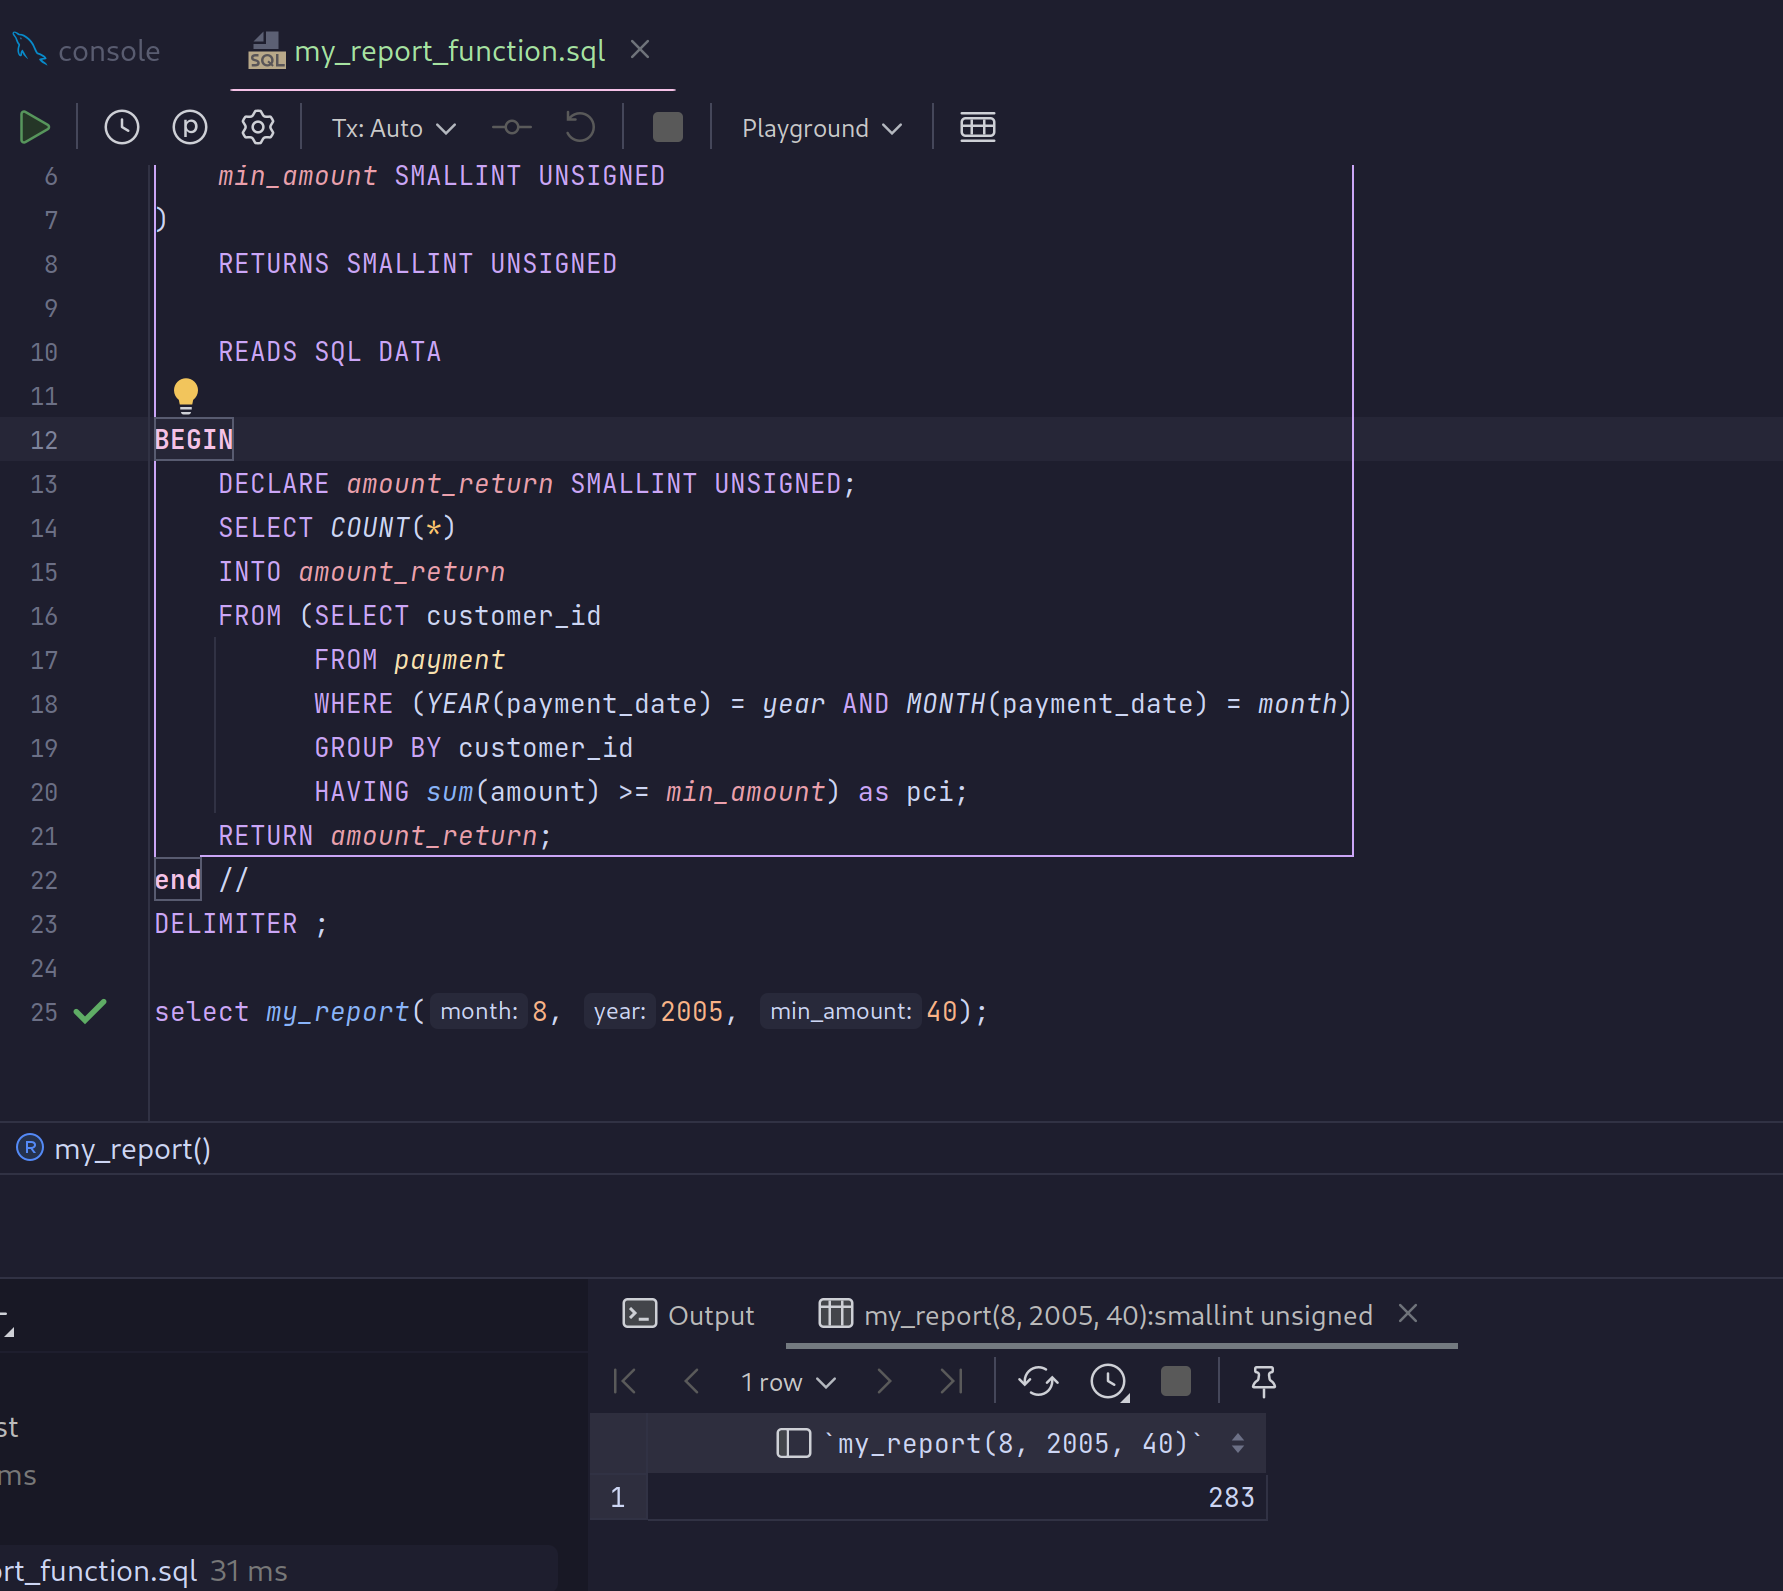
\includegraphics[width=\textwidth, height=\textheight, keepaspectratio]{question1}
	\question
	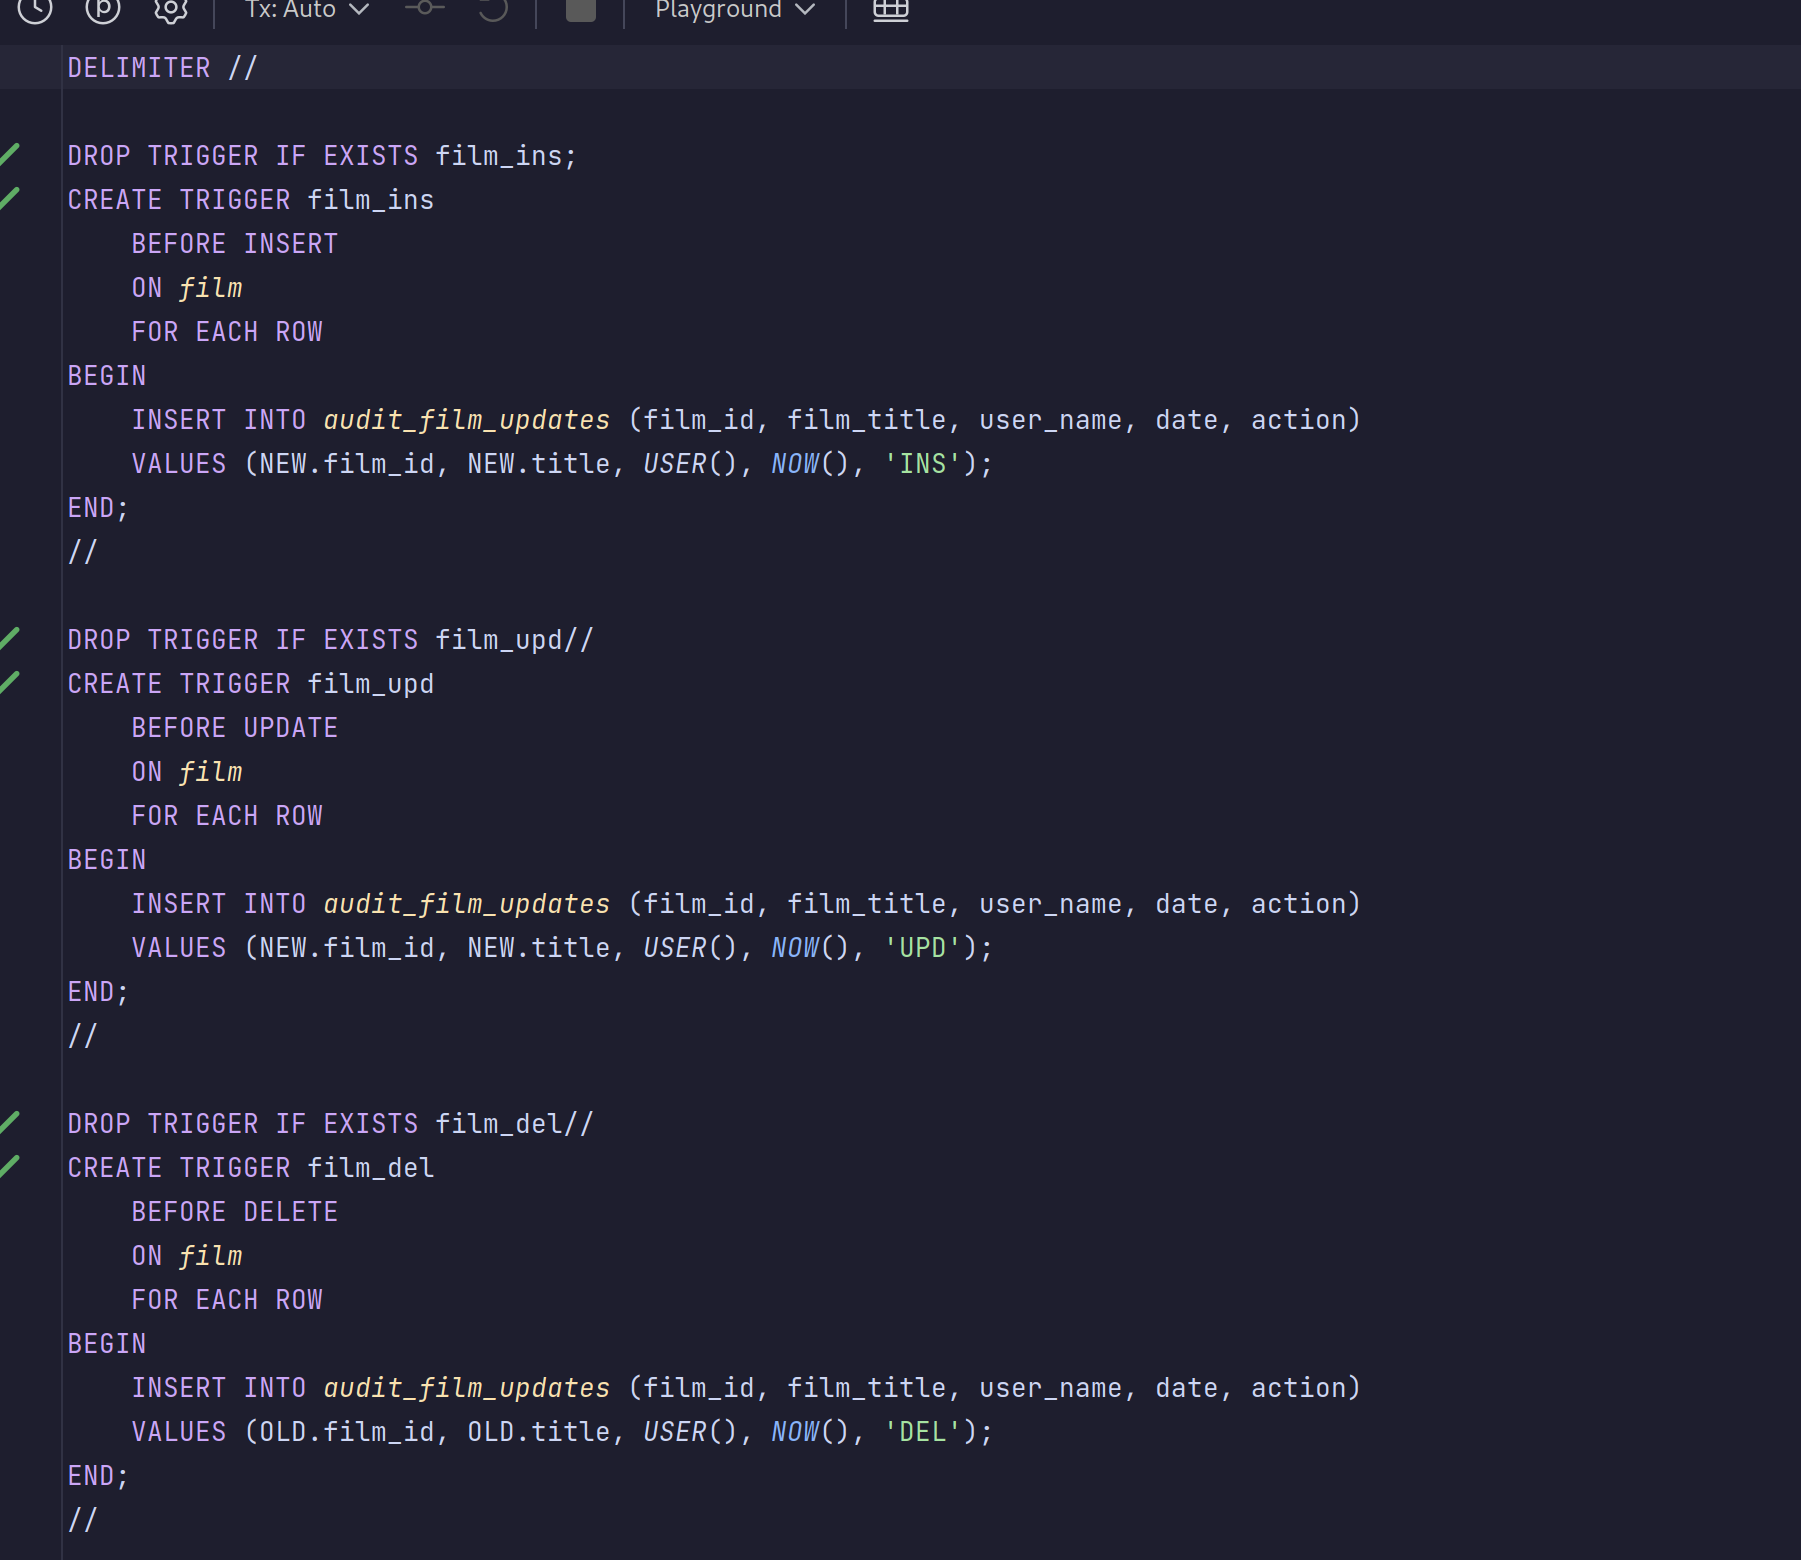
\includegraphics[width=\textwidth, height=\textheight,keepaspectratio]{question2_1}
	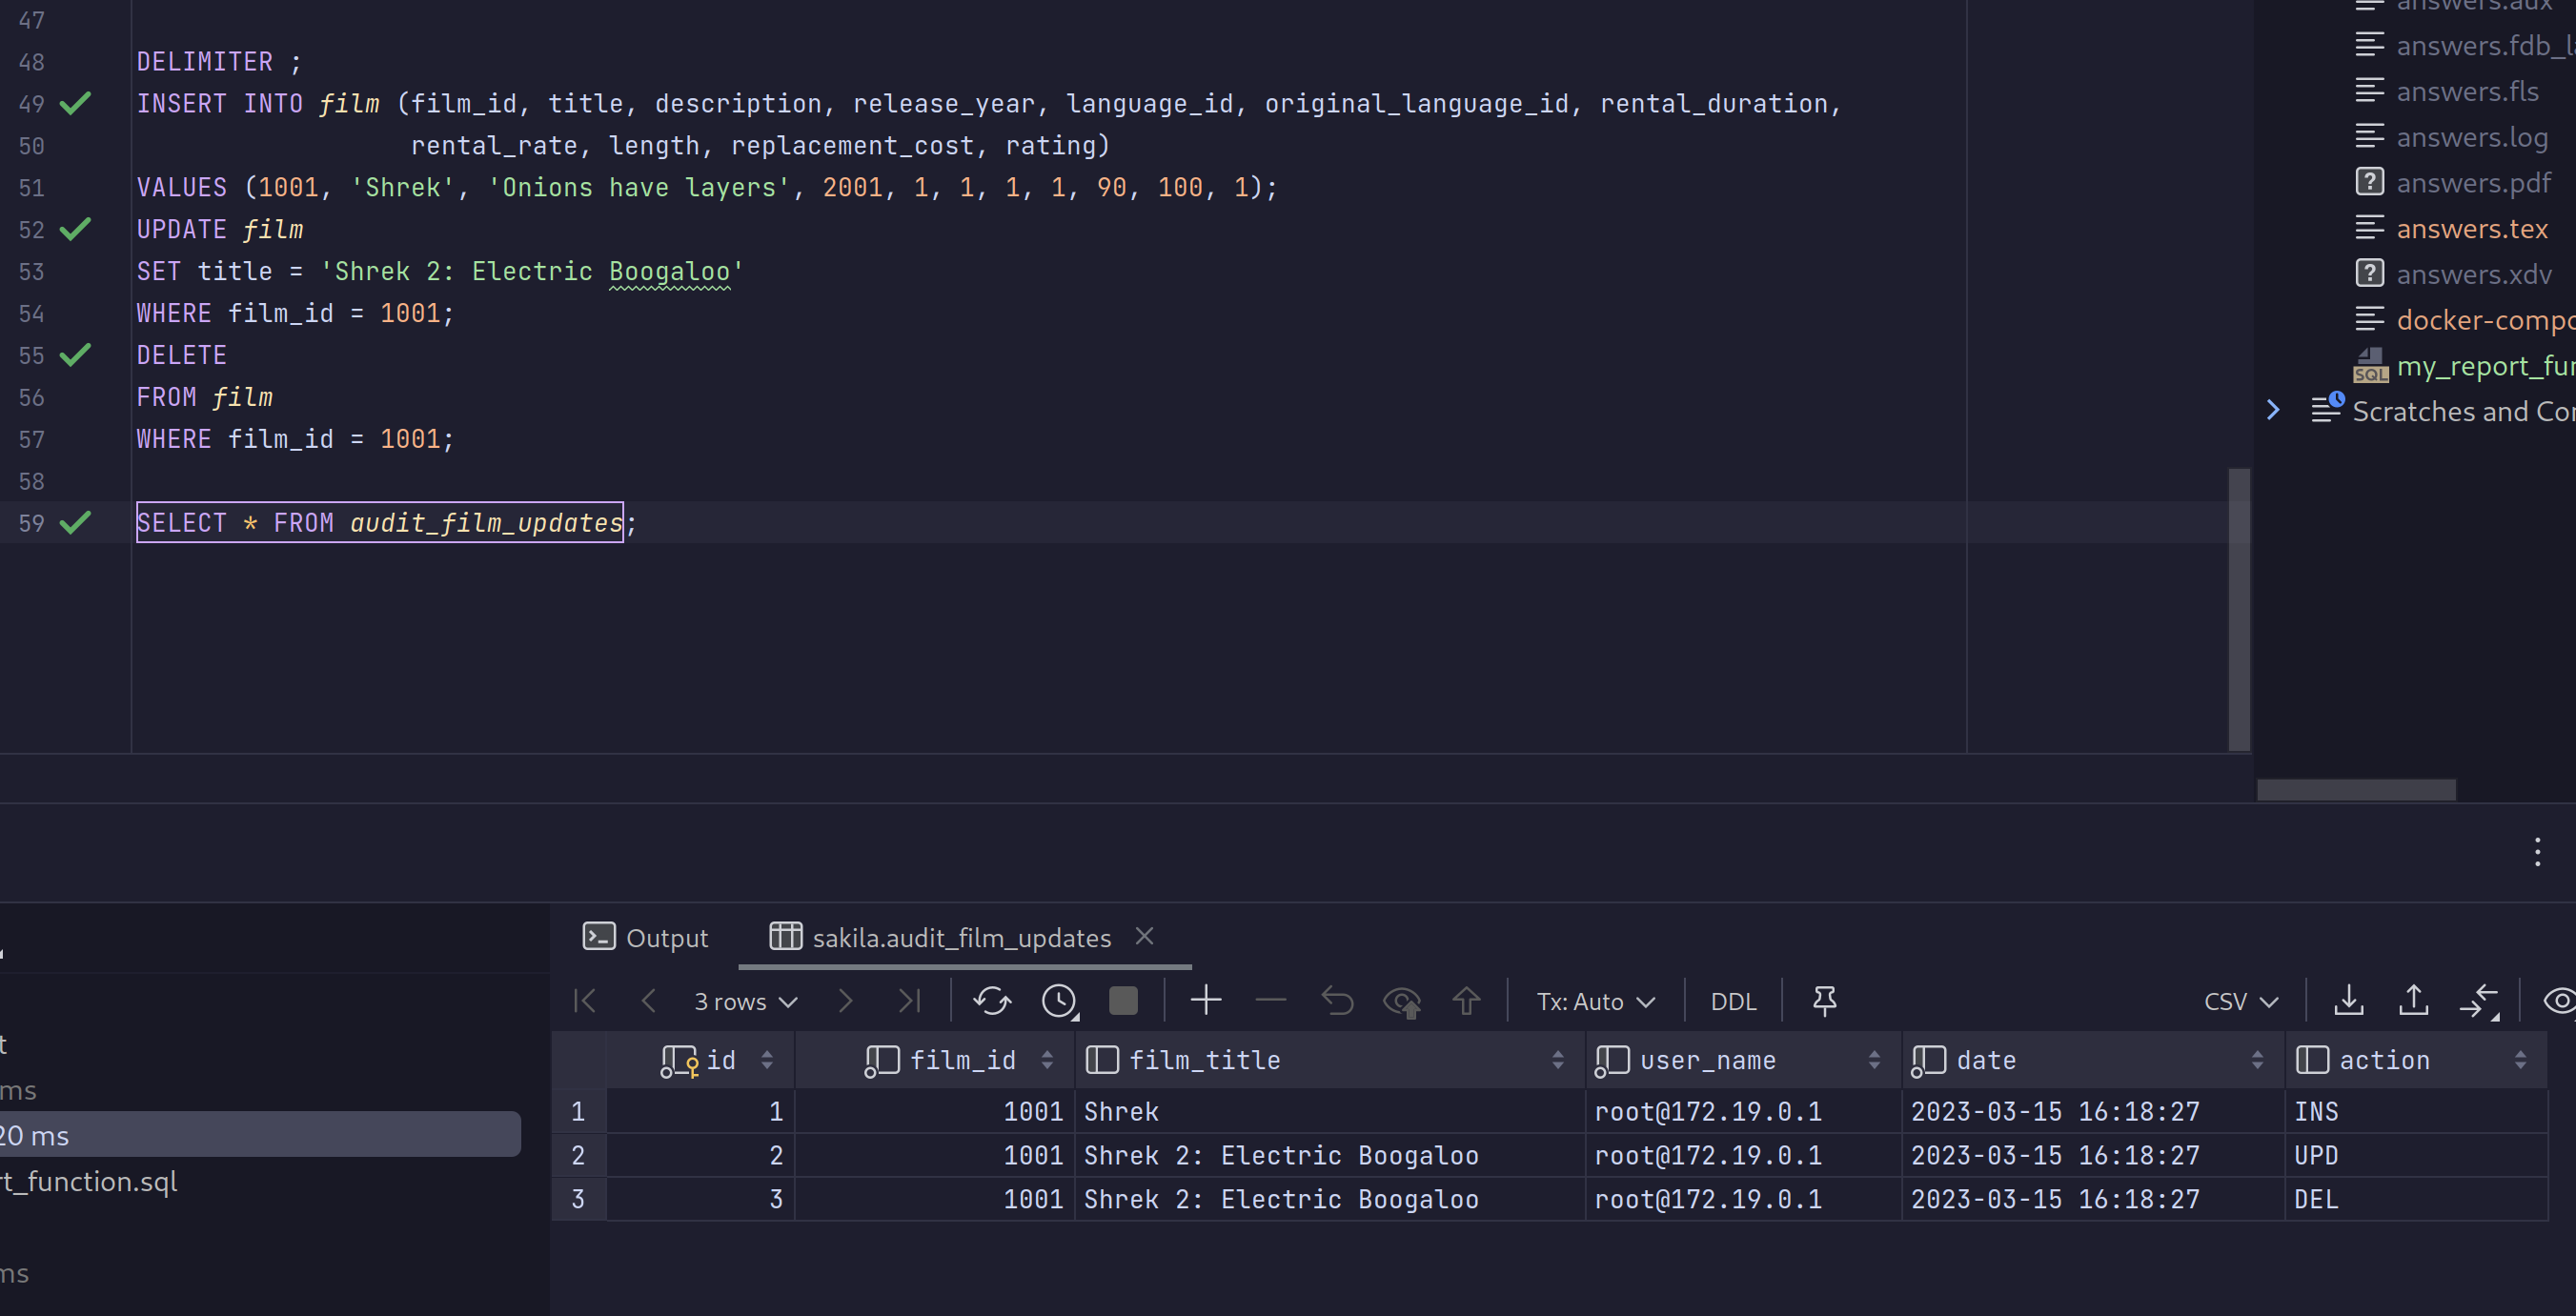
\includegraphics[width=\textwidth, height=\textheight,keepaspectratio]{question2_2}
	\question
	\begin{parts}
		\part
		Een situatie zoals een bank waar geld moet worden afgeschreven en bijgeschreven. Als 1 van beide dingen mislukt kan het voorkomen dat geld wel is afgeschreven maar niet overgemaakt of vice versa.
		\part
		Stel dat twee klanten van een bank een en/of rekening hebben. Als zij beiden tegelijkertijd pinnen wordt er twee keer geld afgeschreven. Echter kan het voorkomen dat er na transactie 1 niet genoeg geld is voor transactie 2. Zonder isolation zou dit een probleem opleveren aangezien beide transacties alsnog gebeuren. De hoeveelheid geld op een bankrekening kan echter(in dit scenario) niet negatief zijn.
	\end{parts}
	\question
	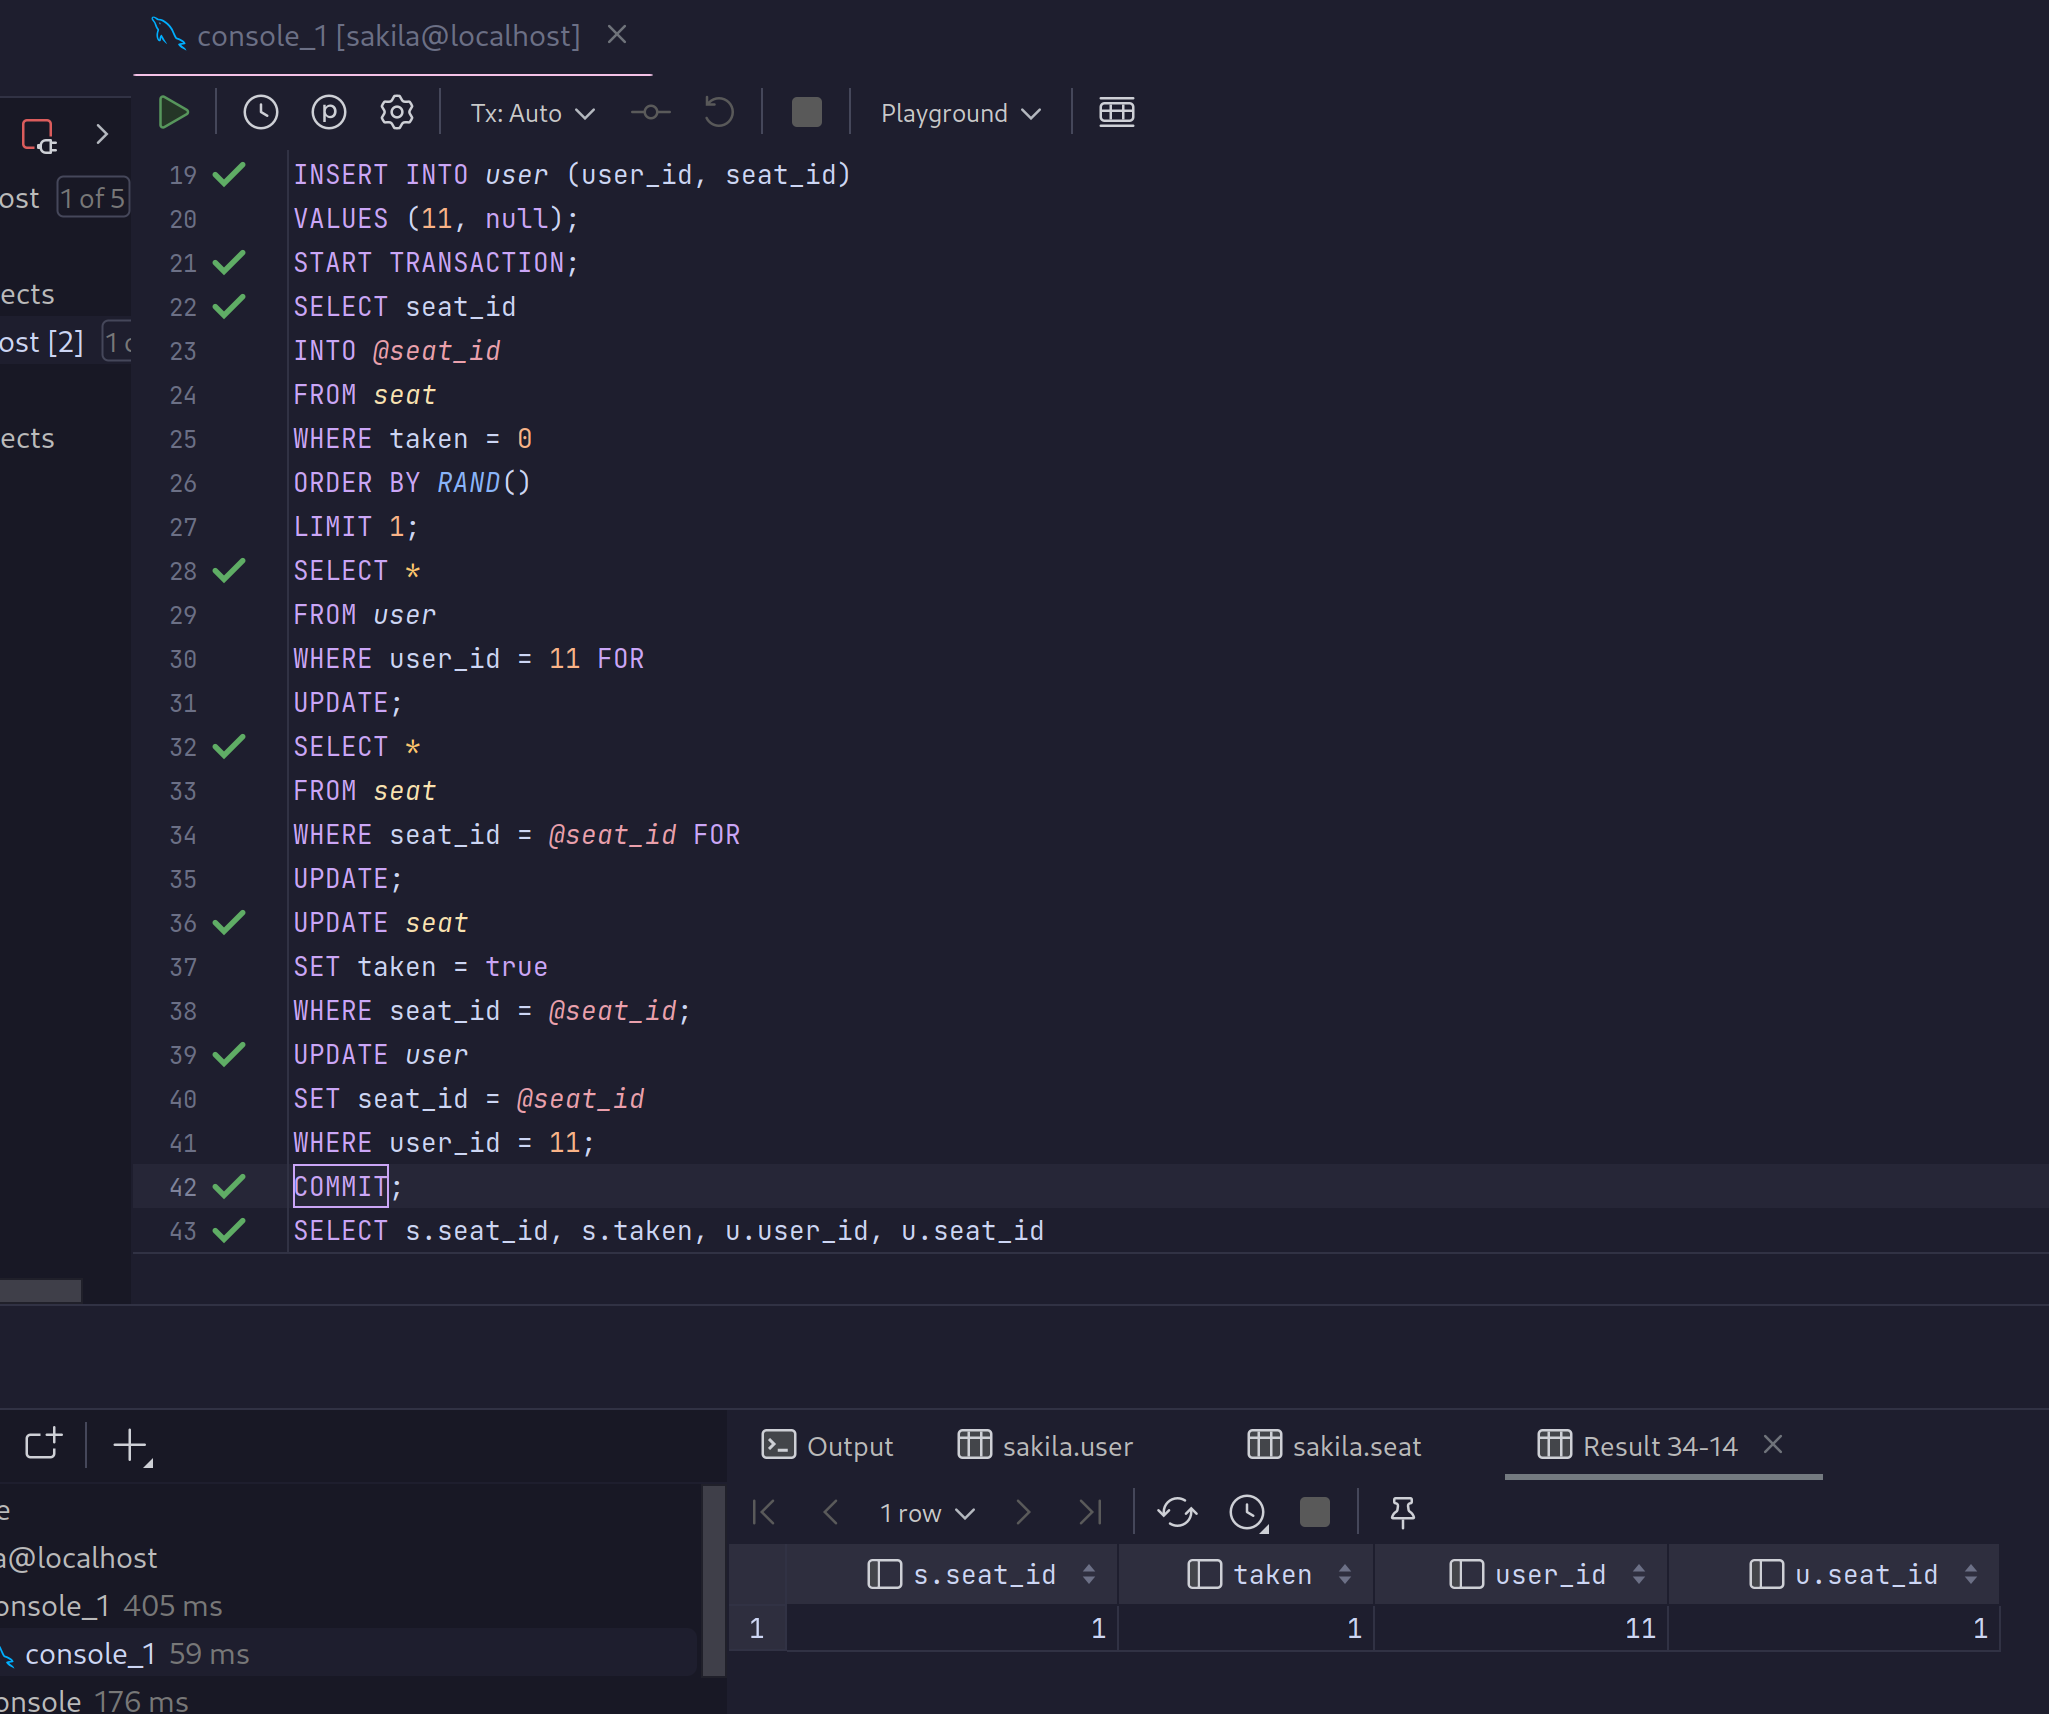
\includegraphics[width=\textwidth, height=\textheight,keepaspectratio]{question4}
	\question
	\begin{tabular}{ |c|c|c| }
		\hline
		scenario & transactie & omschrijving probleem \\
		\hline
		a        & a          & Dirty read            \\
		\hline
		b        & b          & Lost update           \\
		\hline
		c        & b          & Non-repeatable read   \\
		\hline
		d        & a          & Lost update           \\
		\hline
		e        & a          & Dirty read            \\
		\hline
	\end{tabular}
	\question
	\begin{parts}
		\part
		Beide selects zullen een ander resultaat geven, \mintinline{sql}{READ UNCOMMITTED} staat namelijk toe dat er data wordt gelezen die nog niet commited is. In dit geval is er data geupdatet en wordt deze gelezen voordat hij commited is.


		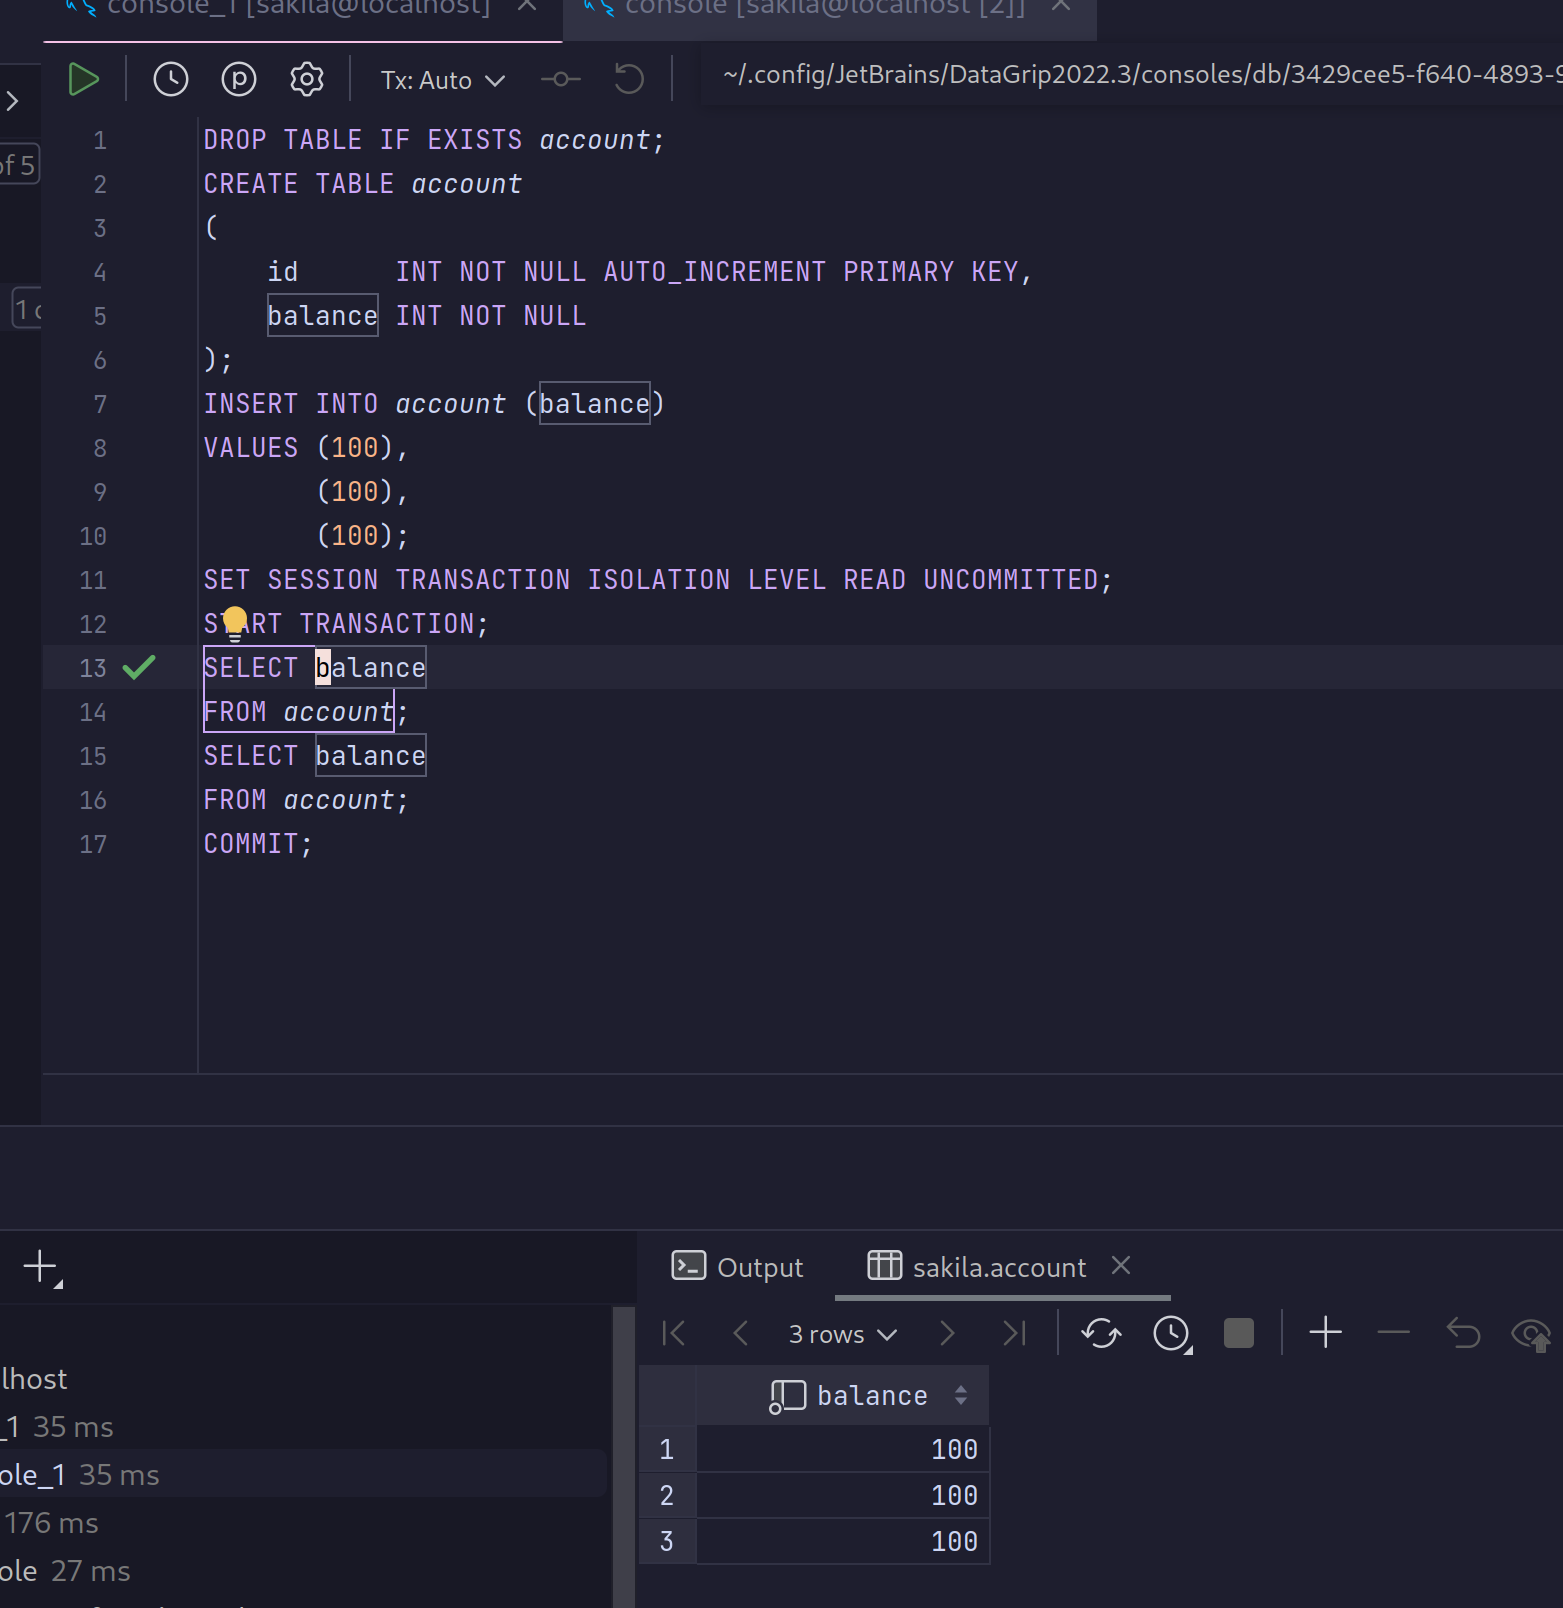
\includegraphics[height=\textheight, width=\textwidth, keepaspectratio]{question6_a_1}
		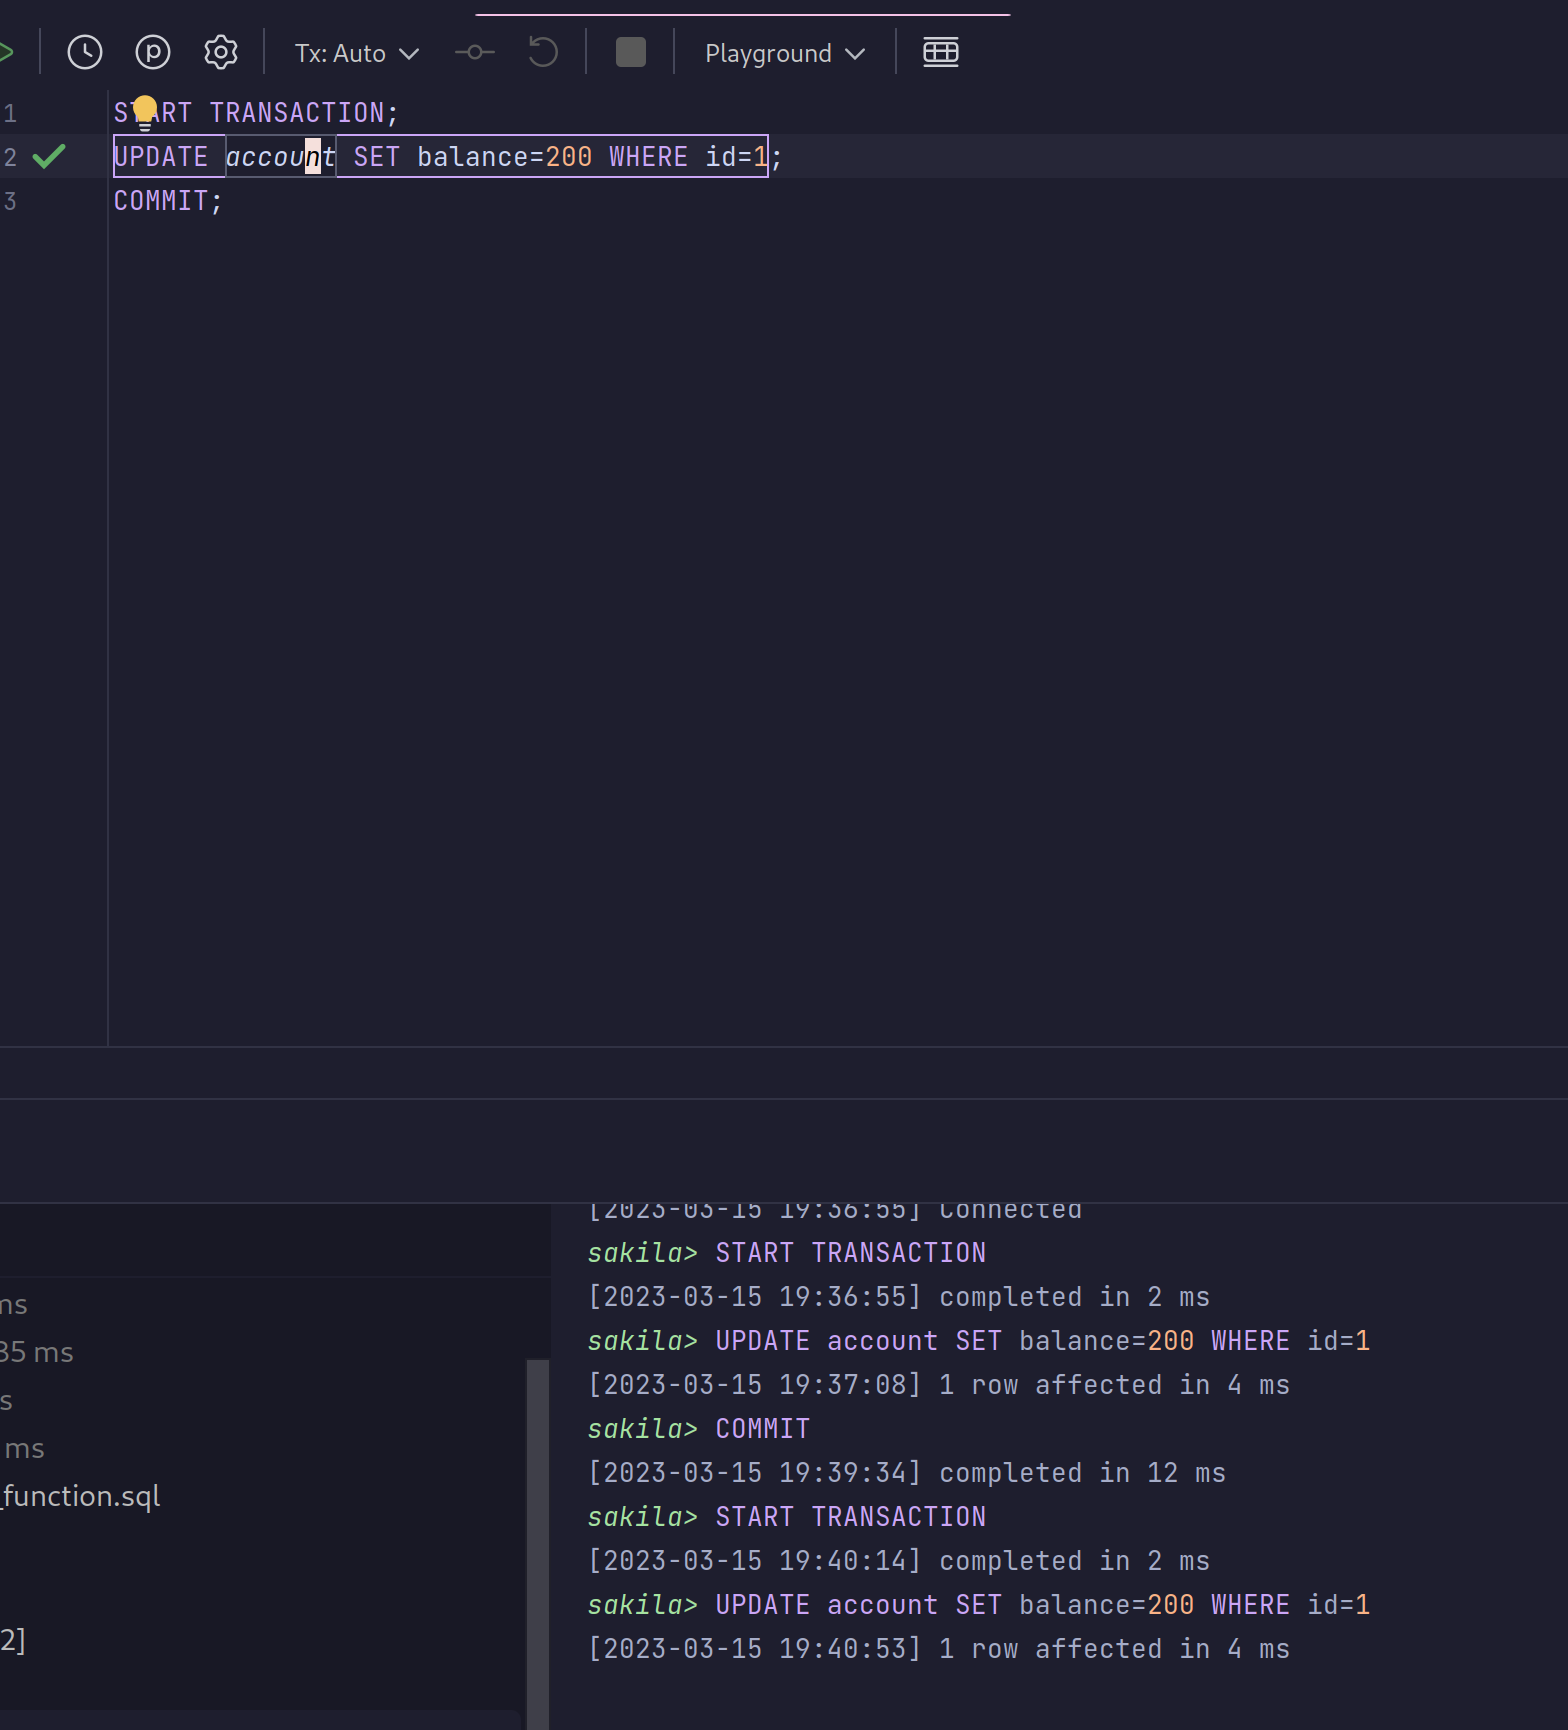
\includegraphics[height=\textheight, width=\textwidth, keepaspectratio]{question6_a_2}
		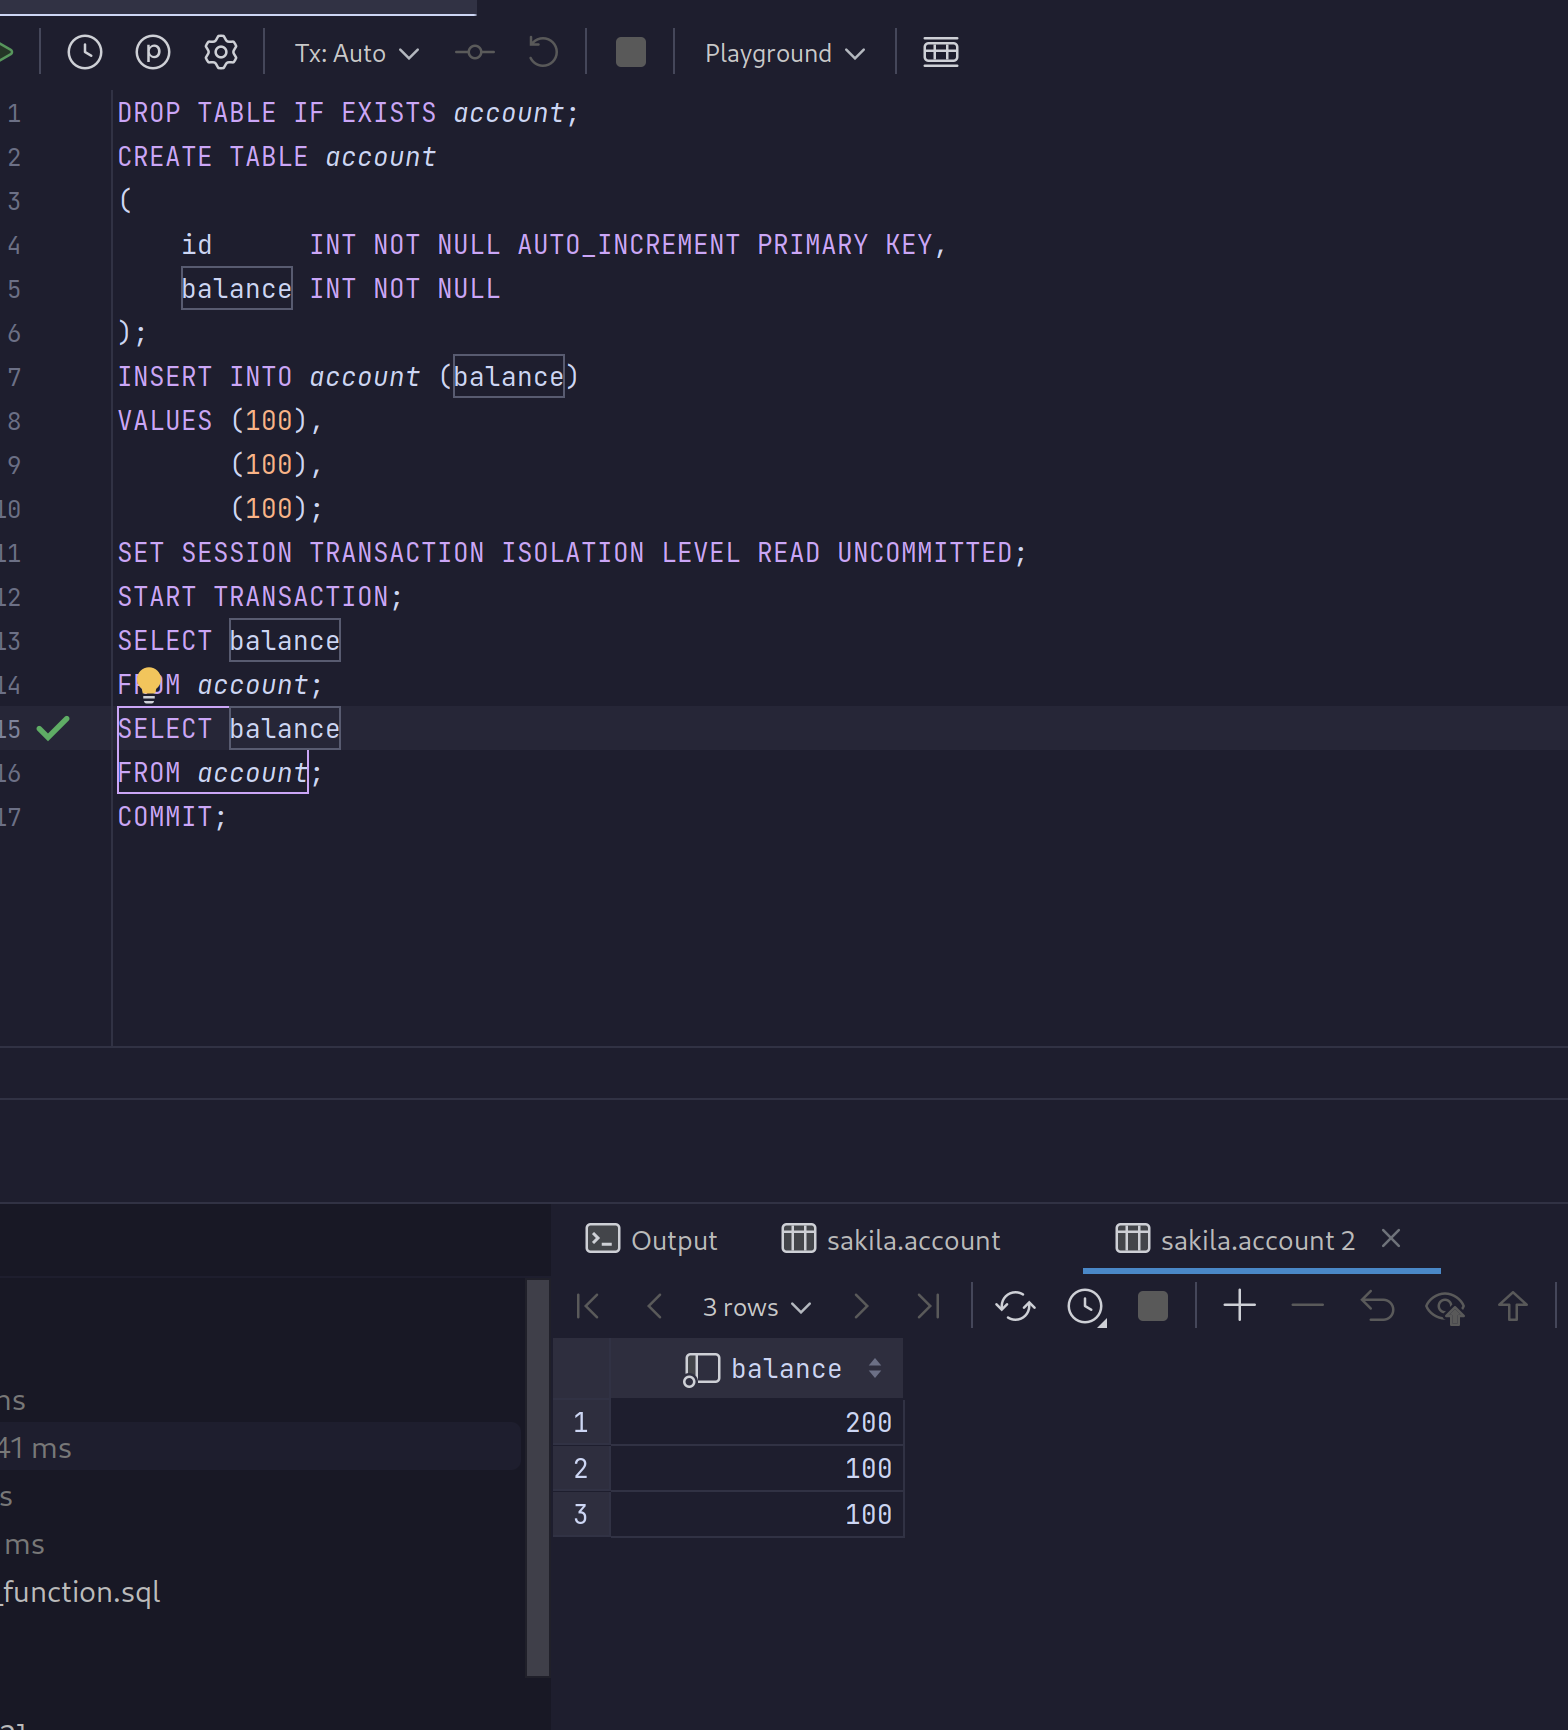
\includegraphics[height=\textheight, width=\textwidth, keepaspectratio]{question6_a_3}
		\part
		De standaard isolation level van MySQL is \mintinline{sql}{REPEATABLE READ} dit voorkomt echter geen phantom reads zoals hierbij het geval is. De twee queries zullen dus alsnog een verschillende result geven.


		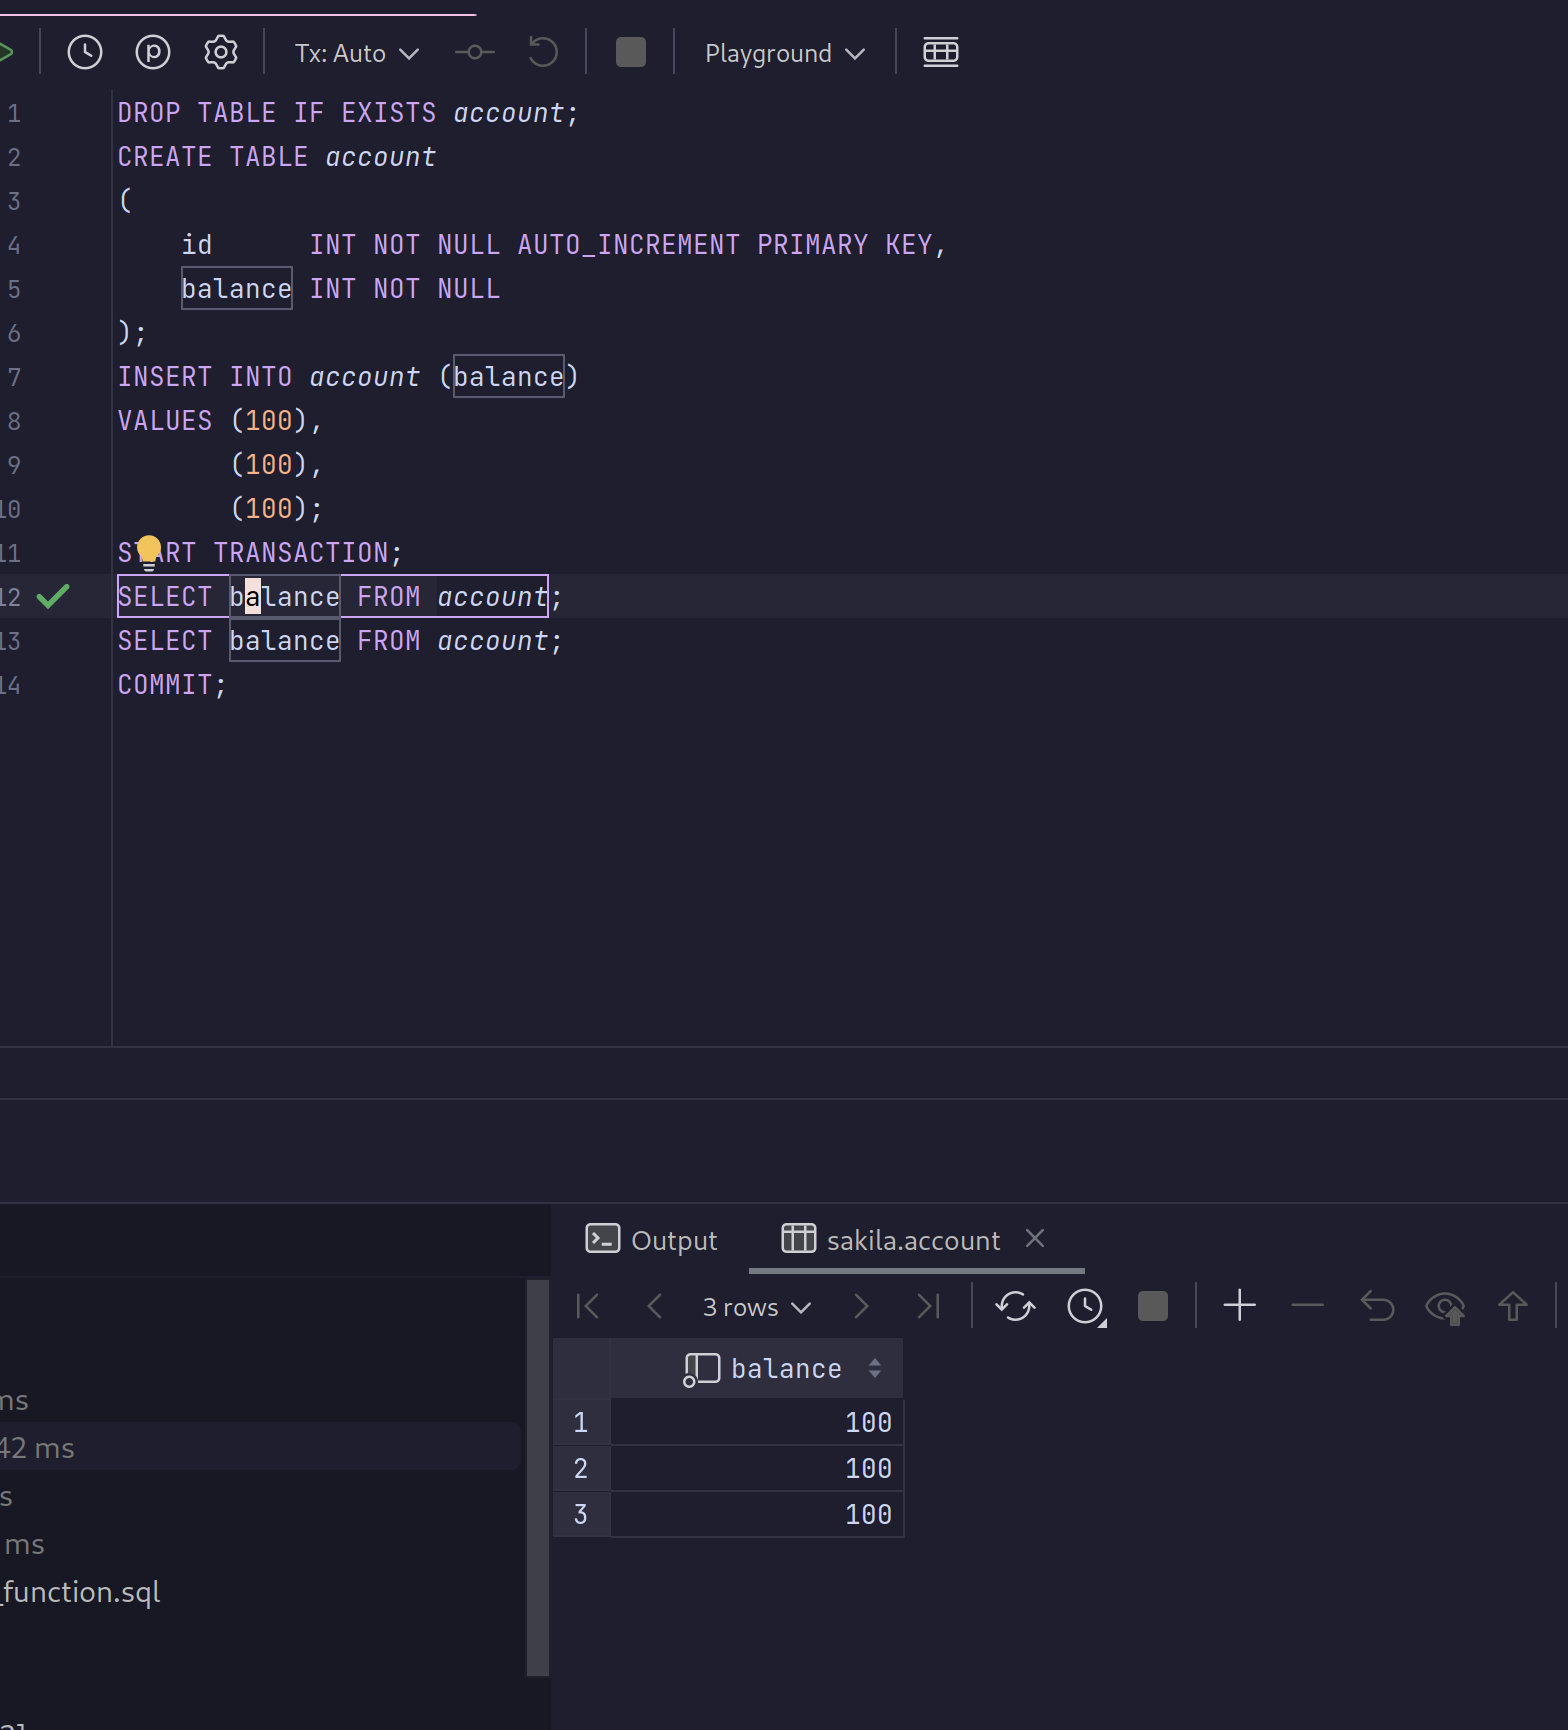
\includegraphics[height=\textheight, width=\textwidth, keepaspectratio]{question6_b_1}
		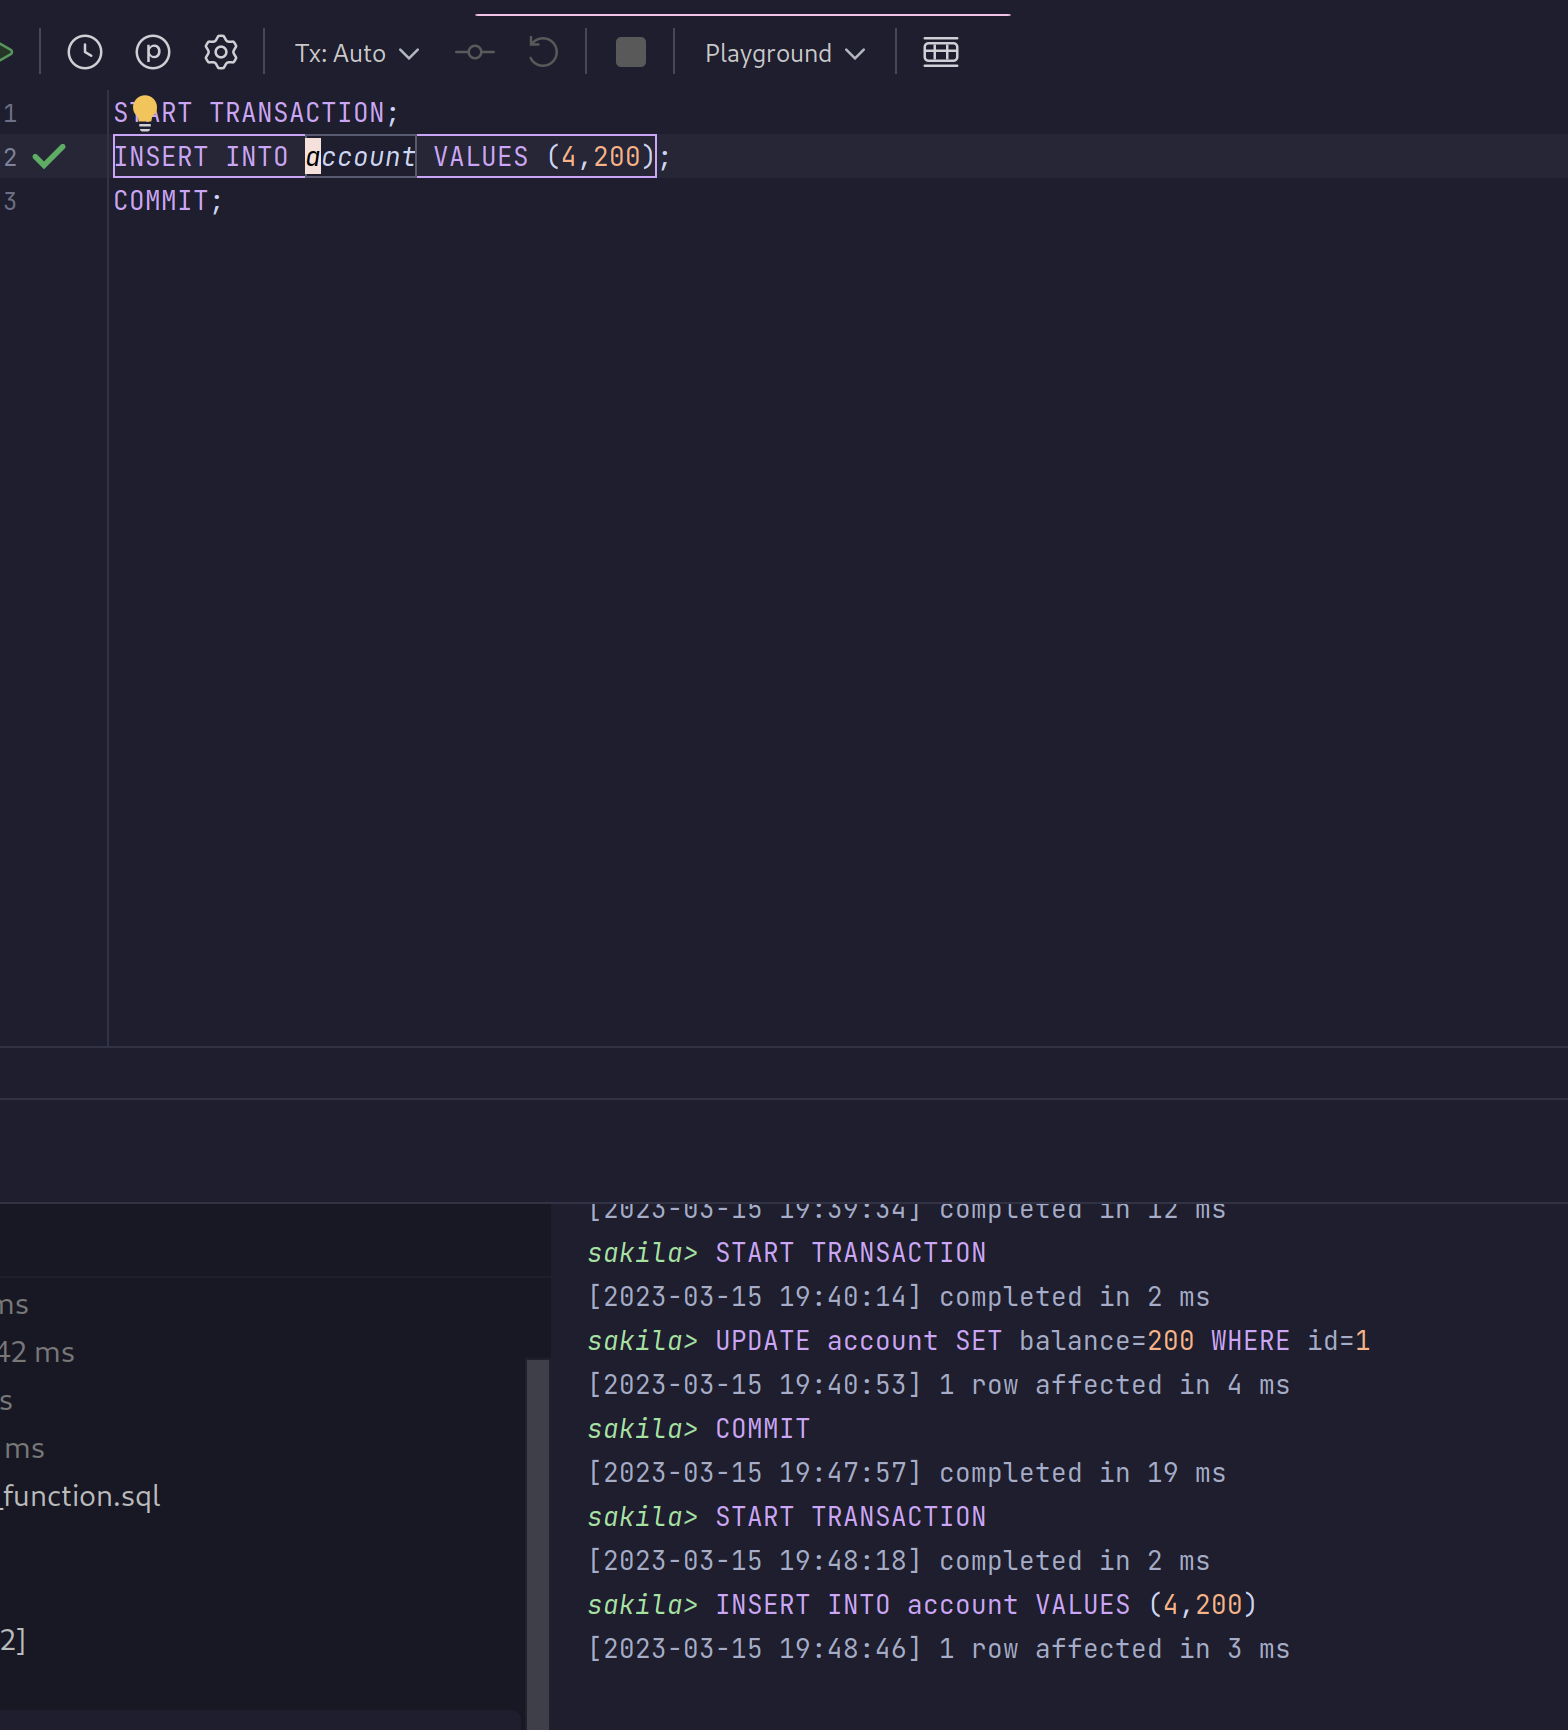
\includegraphics[height=\textheight, width=\textwidth, keepaspectratio]{question6_b_2}
		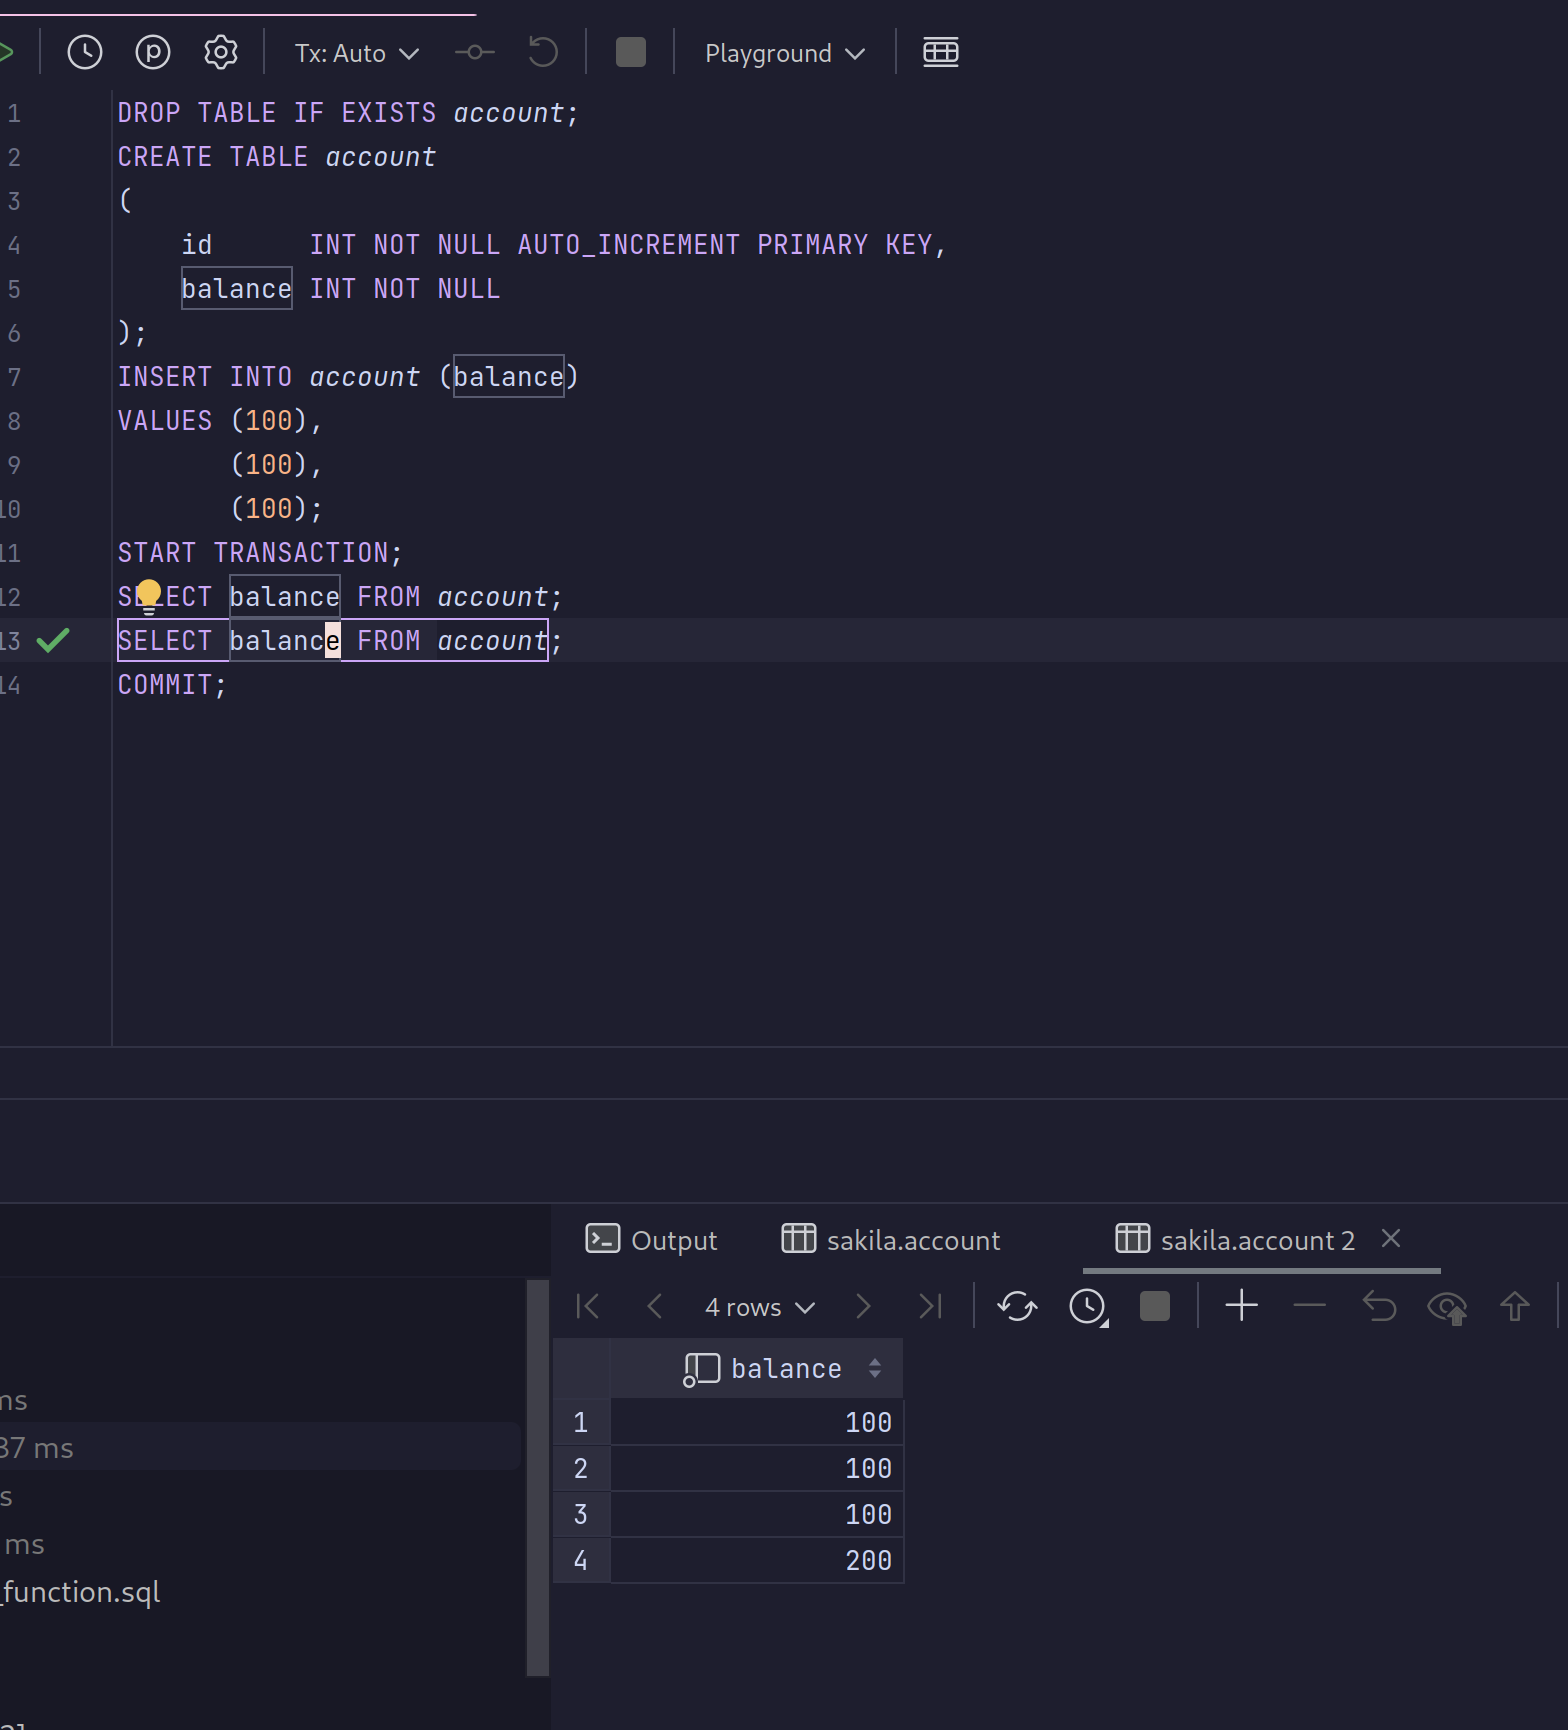
\includegraphics[height=\textheight, width=\textwidth, keepaspectratio]{question6_b_3}
	\end{parts}
	\question
	\begin{parts}
		\part
		Aangezien schrijven exclusieve toegang vereist moet B wachten totdat A klaar is om een lock te krijgen op te krijgen op het object.
		\part
		Door het schrijven heeft A exclusieve toegang. B moet dus wachten totdat deze lock is opgeheven voordat het object kan worden gelezen.
		\part
		Het kan voorkomen dat transacties op elkaar moeten wachten aangezien objects kunnen worden gelockt. Bij MVCC is dit niet het geval en kunnen transacties tegelijkertijd plaatsvinden.
	\end{parts}
	\question
	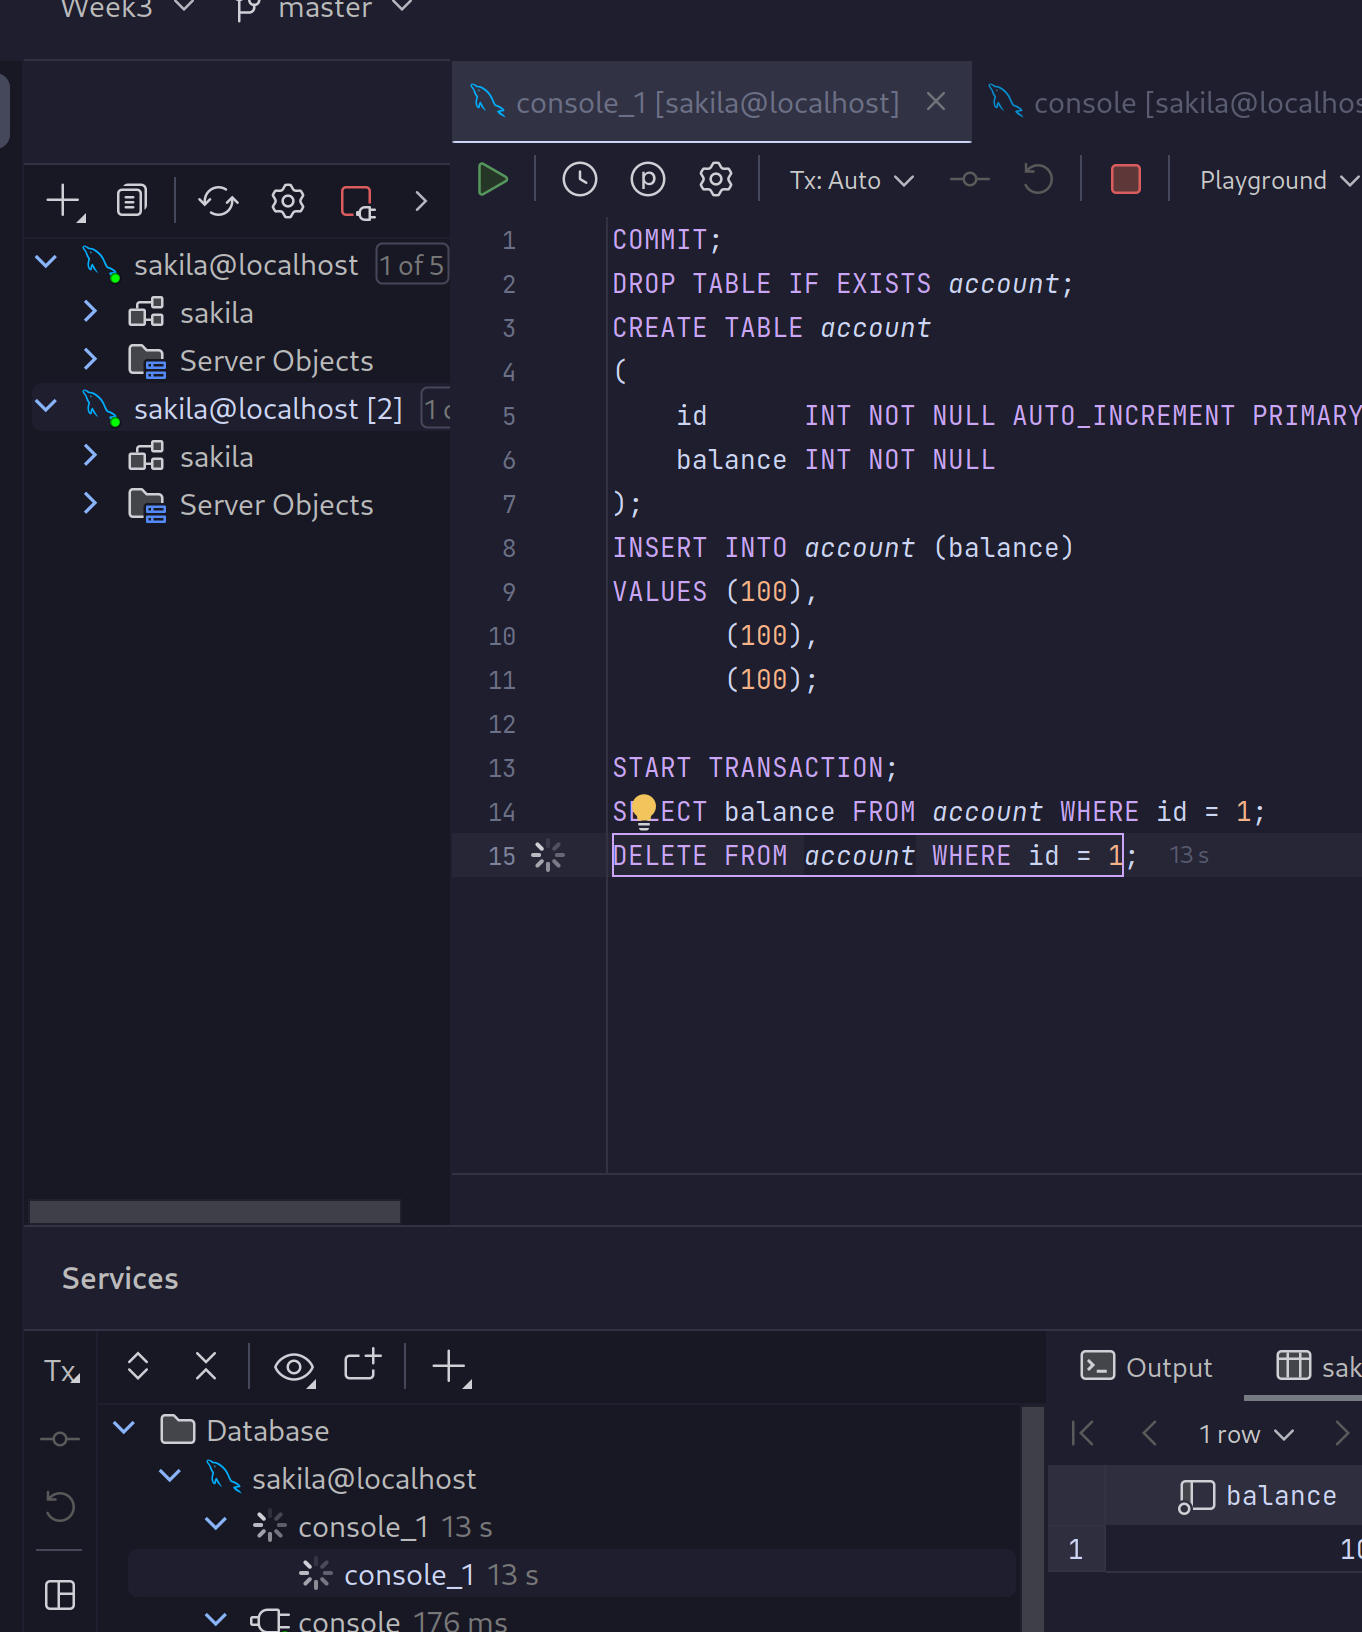
\includegraphics[height=\textheight, width=\textwidth, keepaspectratio]{question8}
\end{questions}


\end{document}
